\documentclass[11pt,a4paper]{article}

\usepackage[utf8]{inputenc}
\usepackage{siunitx}
\usepackage{geometry}
\newgeometry{margin=2.0cm}

\usepackage[backend=biber,style=authoryear,sorting=nyt,dashed=false]{biblatex}
\renewcommand*{\nameyeardelim}{\addcomma\space}
\addbibresource{references/references.bib} % note the .bib is required

\newcommand*\mean[1]{\overline{#1}}
\newcommand\todo[1]{\texttt{#1}}

\title{Effects of Vertical Shear on Cloud Field Variability and Organization }
\author{Mark Muetzelfeldt}
\date{April 2017}

\begin{document}

\maketitle
\section{Introduction}

%\begin{itemize}
%    \item Justification for using RCE - links to QE.
%    \item Motivation for how this work fits into larger picture of stochastic parametrization. Particularly the variability analysis.
%    \item Set out experimental design: choice of shear profiles and explanation of why these produce organization, linking back to previous work, e.g. \cite{RKW1988}.
%    \item Mention: organization and momentum flux.
%\end{itemize}

Most moist convection parametrization schemes in use are deterministic - for a given grid-column state they will produce a single specific amount of convective heating, moistening and perhaps momentum transport. This can be justified through the Quasi-Equilibrium (QE) assumption of \cite{arakawa1974}, in which it is assumed that the convection is in local equilibrium with the grid-scale forcing because each grid-column contains many convective plumes. As model resolution increases, this assumption will breakdown, as each grid-column contains fewer and fewer convective plumes. One way of modelling the parametrized convection in these circumstances is by using a stochastic parametrization scheme - the magnitude of the subgrid convection is not determined by sampling from a Probability Distribution Function (PDF) instead of being uniquely determined by the grid-scale state.

Stochastic parametrization schemes require a characterization of the subgrid variability of the convection. This can be done by using Cloud Resolving Models (CRMs) to verify the theoretical models of how the variability of the convection is distributed. In this study, we look at how the organization of deep convection affects the variability of the convection. In particular, we look at how squall lines consisting generated by deep vertical shear in the troposphere modify the distribution of convective mass flux.

CRMs can exhibit different modes of organization. For example, when run with interactive radiation, CRMs can display self-aggregation. This is where convection develops in a large subregion of the domain, often related to the scale of the model, whilst outside of this region compensating subsidence occurs. The mechanisms for this are disputed, and may be different from model to model. However, interactive radiation, or a prescribed cooling profile that varies across the domain, is necssary. As we with to isolate the organization stimulated by shear, we use a uniform prescribed cooling profile over our domain. This also means we can effectively vary the amount of convection by increasing the magnitude of the cooling.

The simulations carried out are run to statistical equilibrium, in the sense that the model state taken over a large enough domain and time period is statistically indistinguishable from another such period. Thus the model as a whole is [representative?] of the QE assumption. However, at smaller spatial or temporal scales, there will be significant departures from this mean state. It is precisely these fluctuations, and their relative frequencies, that we wish to characterize.

The way we characterize the fluctuations is by investigating the distribution of convective mass flux. Mass flux is a key parameter in convection parametrization schemes, as it value is used to determine the behaviour of a cloud model. This will typically lead to a moistening of the upper troposphere through detrainment from the cloud, as well as a heating of the troposphere, primarily through the compensating subsidence. The magnitude of the mass flux is determined through the use of a closure based on the grid-column state of the model. A popular choice of closure is the Convective Available Potential Energy (CAPE) closure assumption, whereby a percentage of the CAPE is assumed to [be consumed] by the convection in a given timestep. This can be used to set the mass flux by iterating towards the required value or by theoretical arguments. The magnitude of the mass flux then determines how much heating and moistening of the atmosphere will happen because of the unresolved convection, through the use of a cloud model.

\section{Model and experimental design}

\subsection{Model setup}

%\begin{itemize}
%    \item Using an idealized version of the Met Office Unified Model (version 10.7).
%    \item Use resolutions of \SI{1}{km}.
%    \item Running over a domain of 256$\times$256 \SI{}{km^2}, for a duration of \SI{20}{days}. This should be large enough to cover the spatial extent of the squall lines, and long enough to both reach equilibrium and provide a long enough time to average over many squall lines' lifetimes.
%    \item Forced with prescribed cooling of \SI{2}{K.day^{-1}} - typical of radiative cooling rates over the tropics.
%    \item Using a 3D Smagorinsky Turbulence scheme, no convection scheme. Includes the OCF MC scheme.
%    \item Applying a relaxation back to a neutral profile above \SI{12.5}{km} (or \SI{15}{km}?).
%\end{itemize}

The model used is the UK Met Office Unified Model (UM), version 10.7, run in its idealized configuration. It is a fully compressible, non-hydrostatic model, and its dynamics are modelled using a Semi-Implicit Semi-Lagrangian advection scheme. It is run using Cartesian coordinates, over a bi-periodic domain of 256$\times$256 \SI{}{km^2}, using a horizontal resolution of SI{1}{km} and a \SI{30}{s} timestep. It uses a variable vertical resolution, starting at \SI{63}{m} at the surface and increasing to \SI{1}{km} in the stratosphere. 
The experiments are run for \SI{20}{days}, enough time for the simulations to reach equilibrium and for sufficient statistics about the model state to be gathered. The model uses a 3D Smagorinsky subgrid turbulence mixing scheme, with a Richardson based stability function \todo{check}. It includes prognostic ice and graupel in its microphysics, as well as a 2 moment moist microphysics scheme \todo{check/cite}. The surface is treated as ocean, with a fixed temperature of \SI{300}{K} and a roughness length of \SI{0.0002}{m}. The surface heat and moisture fluxes are modelled using bulk aerodynamic formulae, using \todo{values}.

\subsection{Moisture and energy balance}

The SISL advection scheme allows for a large timestep without becoming unstable. Such schemes are not conservative; there is no guarantee that there will be the same total quantity of a tracer from one timestep to the next. In preliminary tests, we found that this had a large impact on the total water content in the model. This lead to precipitation rates being three times higher than what would be expected through comparison with evaporation rates. To ameliorate this, we used the Optimal Conservative Filter (OCF) moisture conservation scheme, developed for previously for this purpose. This scheme is similar to the Priestley scheme, in that it compares the total water content at two consecutive timesteps and ensures conservation by adding or removing water vapour. It does this in a way that is consistent with the uncertainty caused by using interpolation in the SISL scheme, using linear and higher order interpolation as bounds in which it can modify the water vapour in a grid-cell. The OCF scheme differs from the Priestley scheme only in the way it redistributes moisture: it attempts to do it in a way that is locally smooth. With the OCF scheme in use, moisture conservation is guaranteed and once the model has reached equilibrium, precipitation balances evaporation as it should.

In a similar manner to moisture, the SISL scheme can also lead to a non-conservation of energy. No suitable scheme for energy conservation is available in the UM, and so the effects of this energy non-conservation must be characterized and taken into account. This manifests itself as an imbalance between the prescribed cooling energy loss, and the energy input into the model through the surface latent and sensible heat fluxes. Essentially, energy is being supplied by the dynamics of the model, which means that the surface fluxes are less than what would be expected to balance the prescribed cooling by around \SI{50}{W.m-2}.
For the purposes of this study, in which we wish to study the dynamical interactions between clouds, this is not such an issue. This is backed up be the fact that the imbalance mainly affects the stratosphere, i.e. it is far from the area of interest in this study. However, if a detailed energy budget were the focus of an investigation, this would become of prime importance and it would be necessary to either account for the imbalance rigorously, or to apply a similar scheme as the OCF scheme described above to the energy balance. 

\subsection{Initial profiles}

Each simulation is started with an initial moisture and potential profile taken from the final state of a previous reference run. The reference run had a constant mean wind of \SI{5}{m.s-1} across the domain, and was run for \todo{XXX} days until it had reached equilibrium. Simulations are allowed to spin-up for \SI{5}{days} while the surface fluxes come into balance with the energy and precipitation losses from the model. Output from the model is only analysed after the initial spin-up period.

A prescribed cooling rate of \SI{2}{K.day-1} is applied from the surface to \SI{200}{hPa}, decreasing linearly to \SI{0}{K.day-1} by \SI{100}{hPa}. This cooling rate is comparable to typical radiative cooling rates over the tropics. Larger cooling rates representing large-scale convergence and forced ascent, ranging from \SI{4}{K.day-1} to \SI{16}{K.day-1}, were also tested. However, when the model was forced with these rates, it developed a large-scale, domain wide oscillation, thought to be a convectively coupled gravity wave with period equal to the largest scale available to the motion - the length of the domain. These oscillations are a form of organization, and so affect the fluctuations that we are trying to measure. They are also an artefact of the modelling process due to the bi-periodic nature of the boundary conditions, and so are little more than a curiosity and an annoyance. We therefore decided to run with smaller cooling rates that did not stimulate this mode of organization.

\subsection{Shear profiles}

The shear profile that we choose to impose was originally derived from the Marshall Islands experiments \todo{cite}. It has subsequently been used to stimulate mesoscale organization in the form of linear features resembling tropical squall lines, in both 2D \cite{tompkins} and 3D \cite{grabowski, CC2006II} experiments. It is applied by relaxing back to a mean wind across the domain, by applying a single increment to all grid-cells in the domain. In the east-west direction, the increment at each height is given by: $u_{inc} = \frac{U_{ref} - <u>}{\tau} \Delta t$, where $U_{ref}$ is our reference profile, $<u>$ is the domain mean $u$ wind, $\tau = $ \SI{21600}{s}, and $\Delta t$ is the model timestep, or \SI{30}{s}. The reference profile, along with the mean wind from the model over the final day of the simulation, is given in Figure XXX.

%\begin{itemize}
%    \item Profiles are applied by relaxing back to a mean wind across the domain.
%    \item This takes the form of applying an increment of $u_{inc} = \frac{U_{ref} - <u>}{\tau} \Delta t$. $\tau = $ \SI{21600}{s}.
%    \item The momentum flux, can be calculated using $\rho \mean{u' v'} = \rho \frac{u_{inc}}{\Delta t} \Delta z$.
%\end{itemize}

\begin{figure}[htp!]
    \centering
    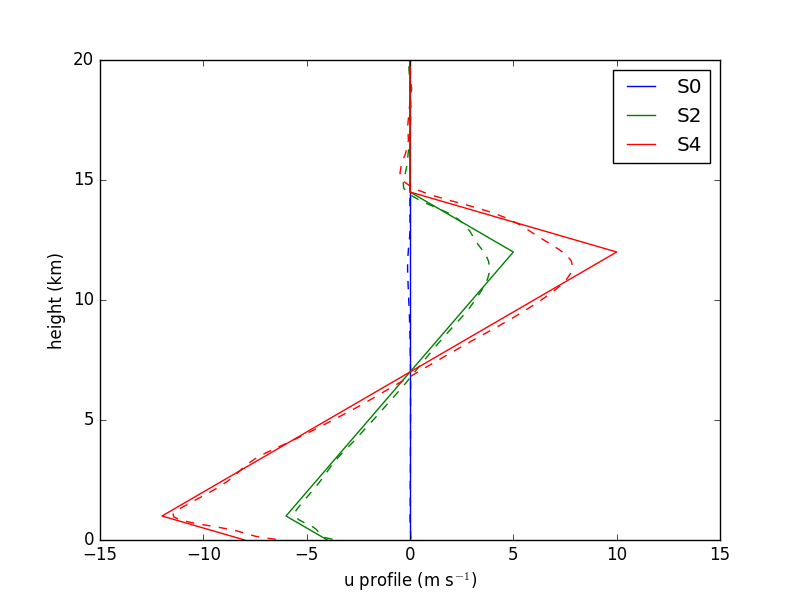
\includegraphics[width=450px]{figs/profile_plot.uv_profile}
    \caption{...}
    \label{fig:MC_on_off}
\end{figure}

\section{Results}
\begin{itemize}
   \item Table 1: List of experiments, S0, S5 etc. plus explanation of each one.

   \item Figure 1: Two snapshots from S0/S5, with no organization and organization present. Something like $w$ at \SI{2500}{m}.
\end{itemize}

\subsection{Spatial variability}
\begin{itemize}
    \item Figure 2: Effects of spatial lengths on total mass-flux (c.f. \cite{PC2008}, Fig. 1).
    \item Figure 3: Effects of spatial lengths on PDF of mass-flux per cloud cell (c.f. \cite{CC2006II}, Fig. 2).
    \item N.B. perhaps combined into one figure.
\end{itemize}

\subsection{Cloud field organization}
\begin{itemize}
    \item Figure 4: Measure of organization demonstrating effectively the higher organization in the organized convection cases.
\end{itemize}

\subsection{Equilibrium profiles}
\begin{itemize}
    \item (Will this be kept?) Figure 5: Difference in equilibrium states from the different experiments. 
\end{itemize}

\subsection{Momentum transports}
\begin{itemize}
    \item Figure 6: Momentum flux profiles for different experiments (c.f. \cite{RE2001}, Fig. 7).
\end{itemize}
\section{Conclusions}

\newpage
\subsection*{Main papers (*:key papers)}
\begin{itemize}
    \item * \cite{CC2006I}
    \item * \cite{CC2006II}
    \item * \cite{RE2001}
    \item * \cite{RKW1988}
    \item * \cite{PC2008}
    \item \cite{birch2014scale}
    \item \cite{cohen2004response}
    \item \cite{gregory1997parametrization}
    \item \cite{houze1977structure}
    \item \cite{kershaw1997parametrization}
    %\item \cite{parker2007simulated}
    \item \cite{robe1996moist}
    \item \cite{sakradzija2016stochastic}
    \item \cite{sengupta1990cumulus}
    \item \cite{TMM1982}
\end{itemize}


\printbibliography[title={References}]


\end{document}
